%    Copyright (C) 2014 Christian T. Jacobs, Alexandros Avdis, Gerard J. Gorman, Matthew D. Piggott.

%    This file is part of PyRDM.

%    PyRDM is free software: you can redistribute it and/or modify
%    it under the terms of the GNU General Public License as published by
%    the Free Software Foundation, either version 3 of the License, or
%    (at your option) any later version.
%
%    PyRDM is distributed in the hope that it will be useful,
%    but WITHOUT ANY WARRANTY; without even the implied warranty of
%    MERCHANTABILITY or FITNESS FOR A PARTICULAR PURPOSE.  See the
%    GNU General Public License for more details.
%
%    You should have received a copy of the GNU General Public License
%    along with PyRDM.  If not, see <http://www.gnu.org/licenses/>.

\documentclass[a4paper,11pt]{report}
\usepackage[margin=1.25in]{geometry}
\usepackage{graphicx}

\setlength{\parskip}{0.25cm}
\setlength{\parindent}{0cm}

\begin{document}

\begin{titlepage}
\begin{center}
\vspace*{3cm}
\huge{PyRDM User Manual}\\\vspace*{2cm}
\LARGE{Version 0.1a-dev}
\end{center}
\end{titlepage}

\tableofcontents

\chapter{Introduction}\label{chap:introduction}
\section{Overview}
PyRDM is a project that focuses on the relationship between data and the scientific software that has either created that data, or operates on that data to create new information. Two examples from geoscience are given for illustrative purposes:
\begin{itemize}
  \item Dispersion of saline solution into an estuary from desalination plant.
  \begin{itemize}
    \item Input data: Bathymetry, atmospheric forcing, etc.
    \item Software: Pre-/post-processing codes; numerical models.
    \item Output data: Provenance; simulated flow fields; diagnostic quantities.
  \end{itemize}
  \item Characterisation of pores media for carbon sequestration.
  \begin{itemize}
    \item Input data: Micro-CT images of rock samples.
    \item Software: Pre-/post-processing of data (e.g. image segmentation, mesh generation); numerical models.
    \item Output data: Provenance; computational meshes that could be used by other flow solvers; computed flow fields; diagnostics.
  \end{itemize}
\end{itemize}

From these two examples one can already start to see a great deal of generality emerging. In order to achieve reproducibility, or indeed computability, one must be able to capture all of the input data (i.e. collected/measured data which should also have its associated provenance). Next the actual software that draws information from that data must be captured, and care must be taken to ensure that the same version that created a particular result from the data is used. Finally, the output data from the software must be captured, including provenance data that details how the input data and software were used to create this new data. PyRDM aims to address these needs by facilitating the automated management and online publication of software and data via citable repositories hosted by Figshare. This library can be incorporated into the workflow of scientific software to allow research output to be curated in a straight-forward manner.

%The \texttt{pyrdm} directory contains a set of modules which can be imported into software-specific tools. The \texttt{bin} directory contains an example of such a tool, designed to publish the Fluidity CFD code and any associated data files to Figshare. Users wishing to 

\section{Licensing}
PyRDM is released under the GNU General Public License. Further details can be found in the COPYING file supplied with this software.

\chapter{Getting started}\label{chap:getting_started}
\section{System requirements}
A standard Python installation is required, as well as any additional Python modules that are listed in the README file under the ``Dependencies'' section. PyRDM is designed to run on the Linux operating system. All development and testing takes place on the Ubuntu Precise (12.04) distribution.

\section{Installation}
It is recommended that users use the terminal to install and run PyRDM. After navigating to the base directory of PyRDM (i.e. the directory that the Makefile is in), use the following command to install the PyRDM library:

  \texttt{make install}

\textbf{Note 1:} \texttt{sudo} may be needed for this if the default install directory is located outside of \texttt{/home}. This will yield a system-wide install of PyRDM.

\textbf{Note 2:} In order for Python to find the PyRDM module, you will need to add the PyRDM base directory to your \texttt{PYTHONPATH} environment variable, unless you have used \texttt{sudo} as mentioned in Note 1 above. This can be achieved using:

  \texttt{export PYTHONPATH=\$PYTHONPATH:/path/to/pyrdm}

You may wish to add this statement to your \texttt{/home/your\_username/.bashrc} or \texttt{/etc/bash.bashrc} files so the \texttt{PYTHONPATH} is set correctly each time you log in.

\section{Configuration}
You should copy the contents of the file \texttt{pyrdm.ini.example} to a new file called \texttt{pyrdm.ini} and save it in the \texttt{/home/your\_username/.config} directory. If this directory does not exist, please create it first using

  \texttt{mkdir /home/your\_username/.config}

The contents of the new file \texttt{pyrdm.ini} should then be modified as per the guidance in the following subsections.

\subsection{GitHub repository}
The URL (including the \texttt{http://} prefix) and the name of the GitHub repository which hosts the scientific software should be provided under the \texttt{github} section of the configuration file.

\subsection{Figshare authentication}\label{sect:authentication}
PyRDM requires a set of authentication details in order to publish and modify files using your Figshare account. You will need to login and use the Figshare web interface to generate these authentication details, after which you should paste them into the \texttt{figshare} section of the configuration file.

\begin{enumerate}
  \item Go to \texttt{http://figshare.com/account/applications}
  \item Click \texttt{Create a new application}
  \item Fill in the application details as per Figure \ref{fig:application_details}
  \item Ensure that the application has read and write access to your Drafts, Private and Public articles, as per Figure \ref{fig:permissions}
  \item Click \texttt{Save changes}. PyRDM should appear in your list of applications which can access your account.
  \item Click \texttt{View} next to PyRDM and then click the \texttt{Access codes} tab to see the authentication details. The four fields should be pasted into the \texttt{pyrdm.ini} configuration file.
\end{enumerate}

\textbf{Note:} If you are publishing through a group account, you will need to ask the account's administrator for the authentication details.

\begin{figure}
  \centering
  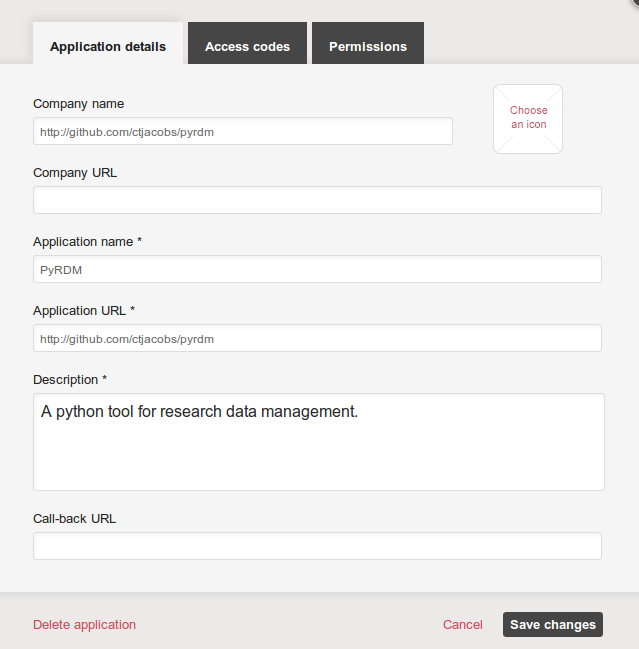
\includegraphics[width=1\columnwidth]{images/application_details.png}
  \caption{The application details for PyRDM.}
  \label{fig:application_details}
\end{figure}

\begin{figure}
  \centering
  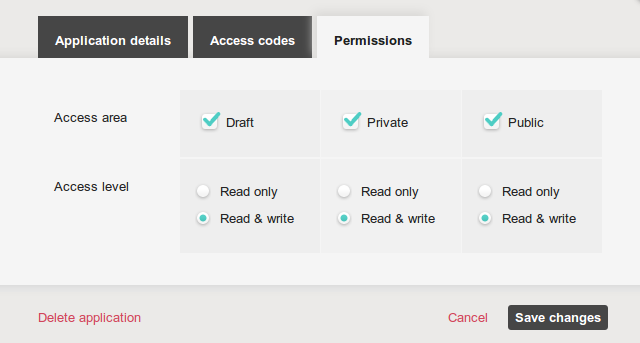
\includegraphics[width=1\columnwidth]{images/permissions.png}
  \caption{The set of permissions required by PyRDM.}
  \label{fig:permissions}
\end{figure}

\section{Testing}
PyRDM comes with a suite of unit tests which verify the correctness of its functionality. It is recommended that you run these unit tests before using PyRDM by executing:

  \texttt{make unittest}
  
on the command line. Many of these tests require access to a Figshare accont, so please ensure that the \texttt{pyrdm.ini} setup file contains valid Figshare authentication tokens.

\chapter{Publishing}

\section{Publishing software}
The publication of software is handled by the \texttt{publish\_software} method in the Publication class. This requires:

\begin{itemize}
  \item The Figshare authentication details (see Section \ref{sect:authentication}).
  \item The software's name.
  \item The version of the software that you would like to publish (for GitHub repositories, this is the SHA-1 commit hash).
  \item The location of the software's Git repository (or the location of any file within that repository) on your local hard drive.
\end{itemize}

\subsection{Author attribution}
If an AUTHORS file is provided in the Git repository's base directory, PyRDM parses it and looks for strings of the form figshare:xxxx, where xxxx is an author ID. Author IDs should be specified after each author's full name. An example is: 

\texttt{Christian Jacobs (figshare:554577)}

PyRDM automatically adds all authors who provide their Figshare author IDs to the software publication.

\section{Publishing data}
The publication of software is handled by the \texttt{publish\_software} method in the Publication class. This requires:

\begin{itemize}
  \item The Figshare authentication details (see Section \ref{sect:authentication}).
  \item A dictionary of parameters, containing the following key-value pairs:
    \begin{itemize}
      \item \texttt{title}: the title of the dataset
      \item \texttt{description}: a description of the dataset
      \item \texttt{files}: a list of paths to the files within the dataset.
    \end{itemize}
  \item Optionally, an \texttt{article\_id} if the dataset already exists on the Figshare servers and you wish to update it. By default, this is set to \texttt{None}.
\end{itemize}

\subsection{MD5 cross-checks}
When a data file is published, the file's MD5 checksum is stored in a corresponding checksum file. The next time the user tries to publish the file, its MD5 checksum is recomputed and compared against the MD5 checksum stored in its corresponding MD5 file. If the two MD5 checksums are different (or the checksum file does not exist), the file is uploaded to the Figshare server and the checksum file is updated with the new checksum. If the two checksums are the same, the file is unmodified and is not re-uploaded. This can help prevent unnecessary bandwidth usage and is particularly useful when you have large data files which are not frequently modified.

\end{document}
